\documentclass[a4paper,10pt]{article}

% Hier die Nummer des Blatts und Autoren angeben.
\newcommand{\blatt}{7}
\newcommand{\autor}{Alexander Hildebrandt}

\usepackage{hci}

\begin{document}
% Seitenkopf mit Informationen
\kopf
\renewcommand{\figurename}{Figure}

\aufgabe{10}

\begin{figure}[ht]
\centering 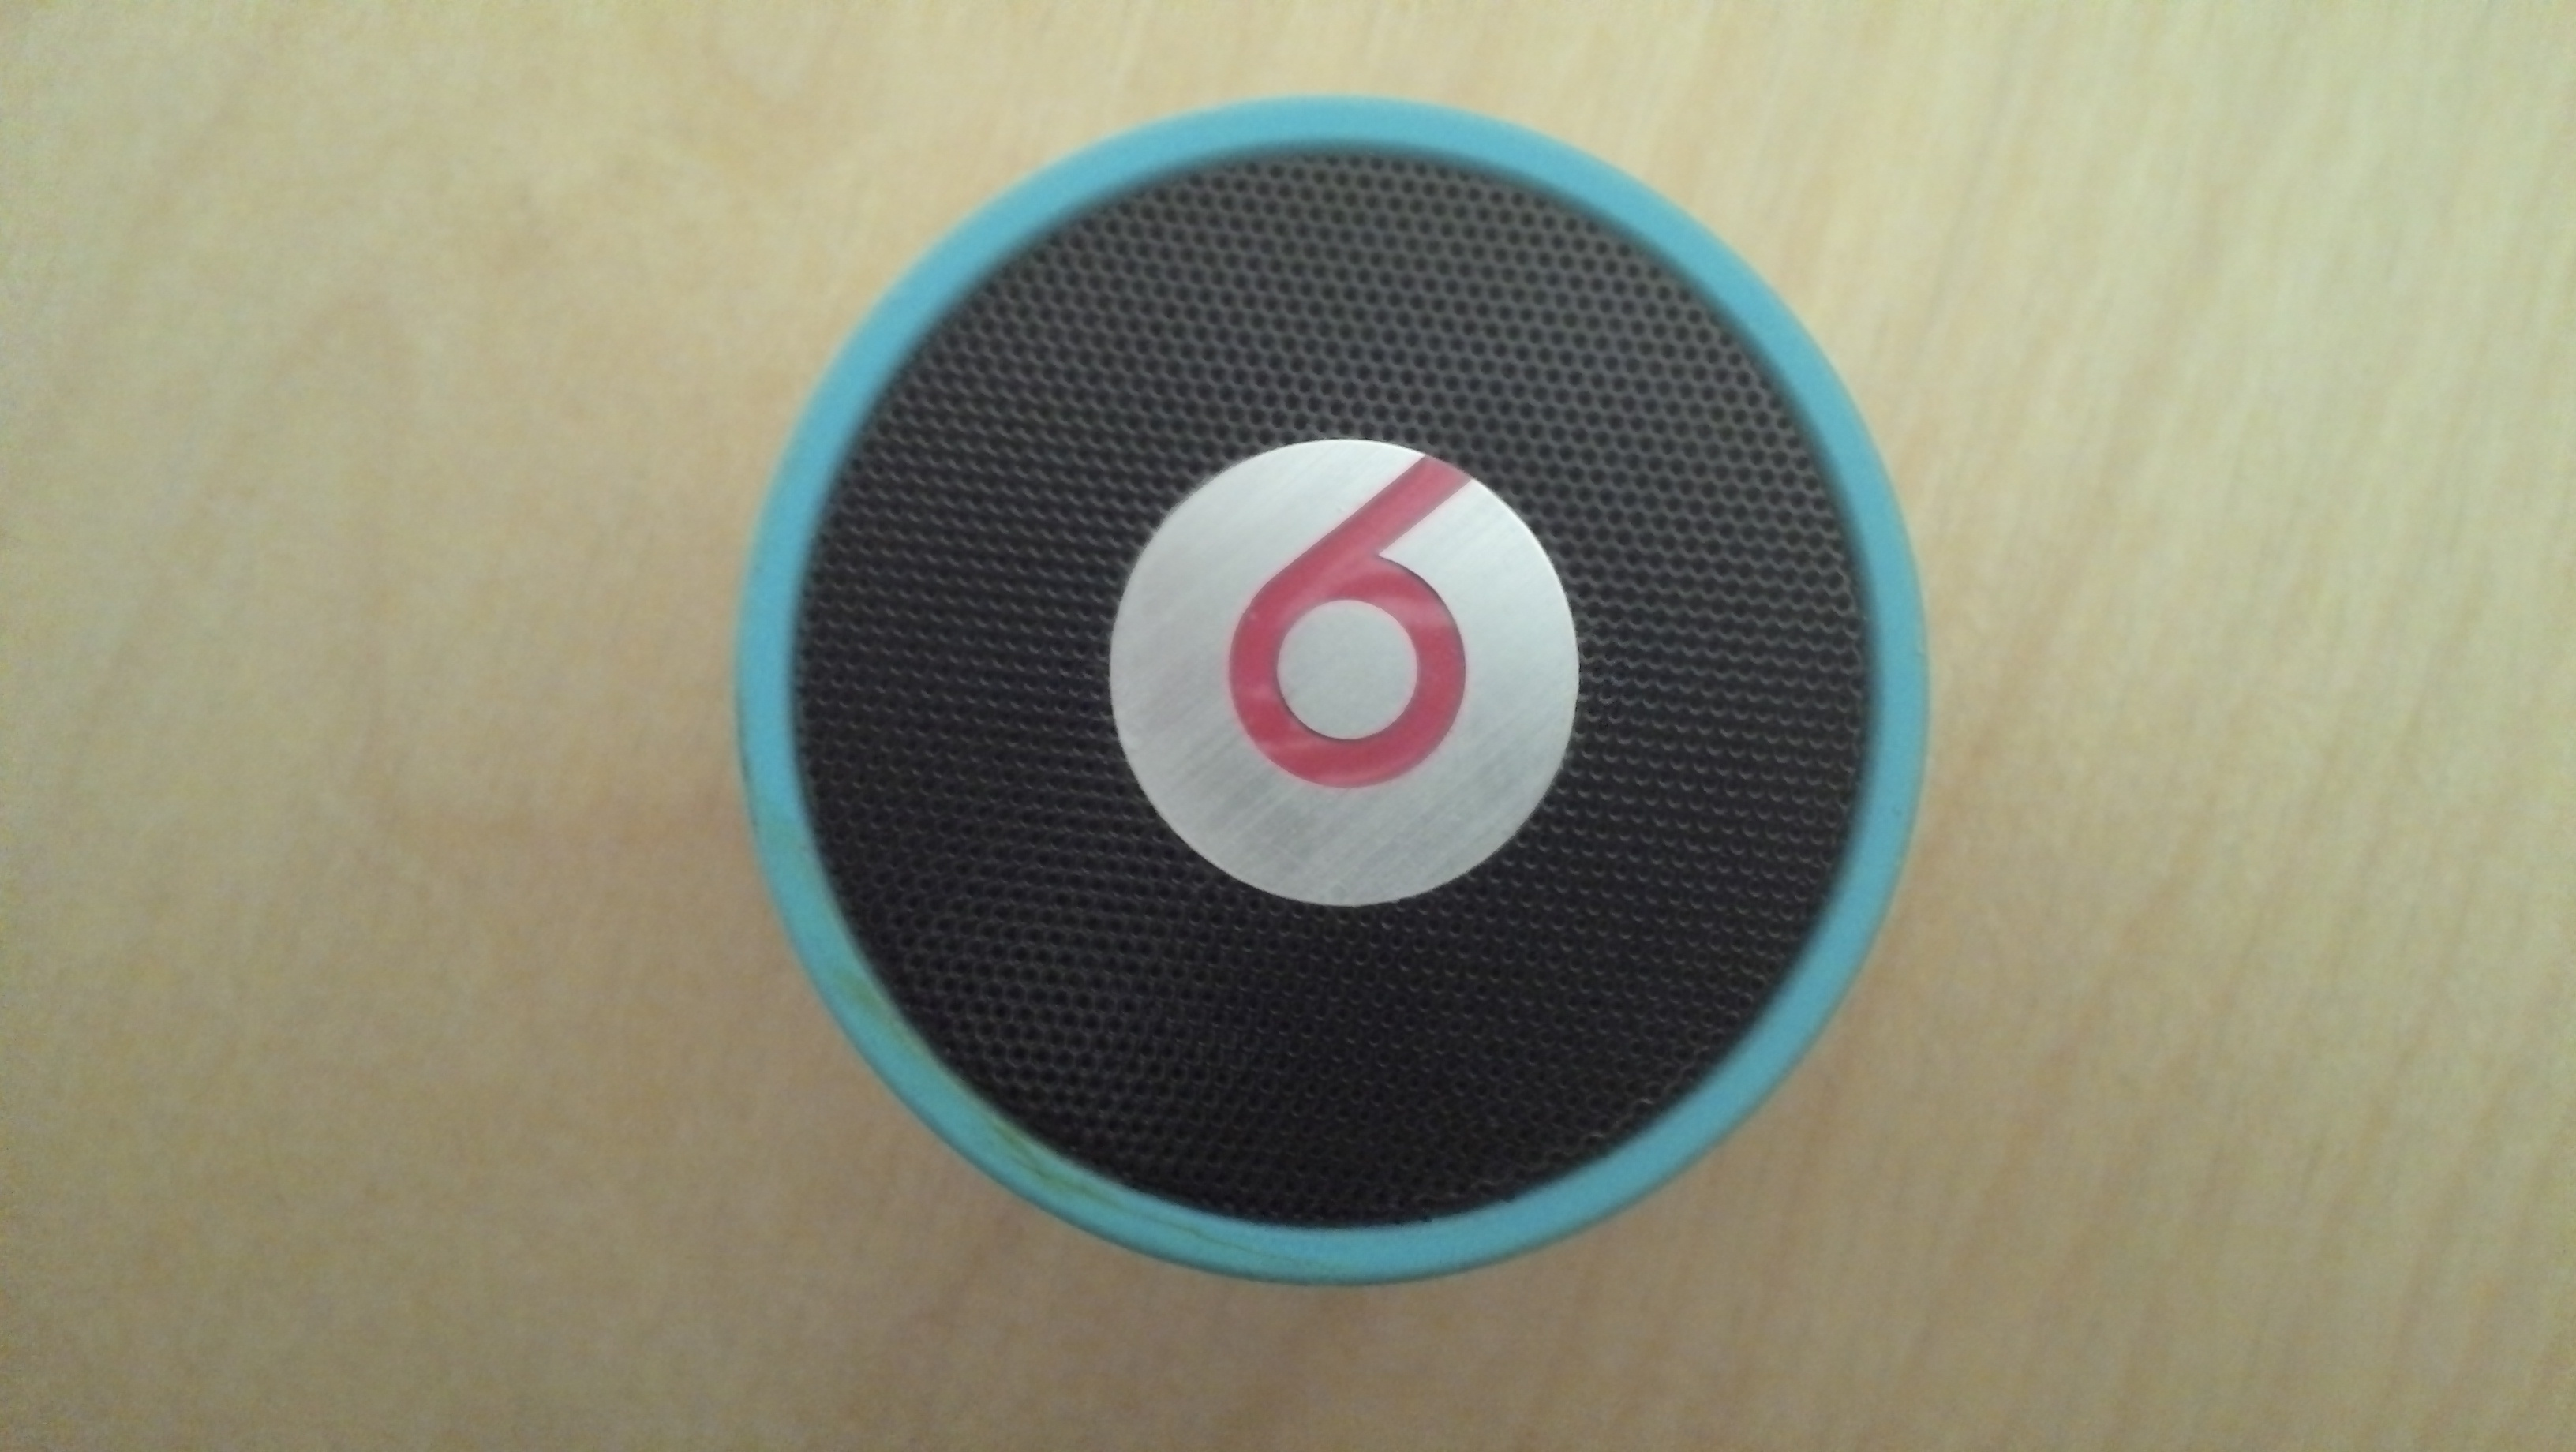
\includegraphics[width=1\textwidth]{pic1.jpg}
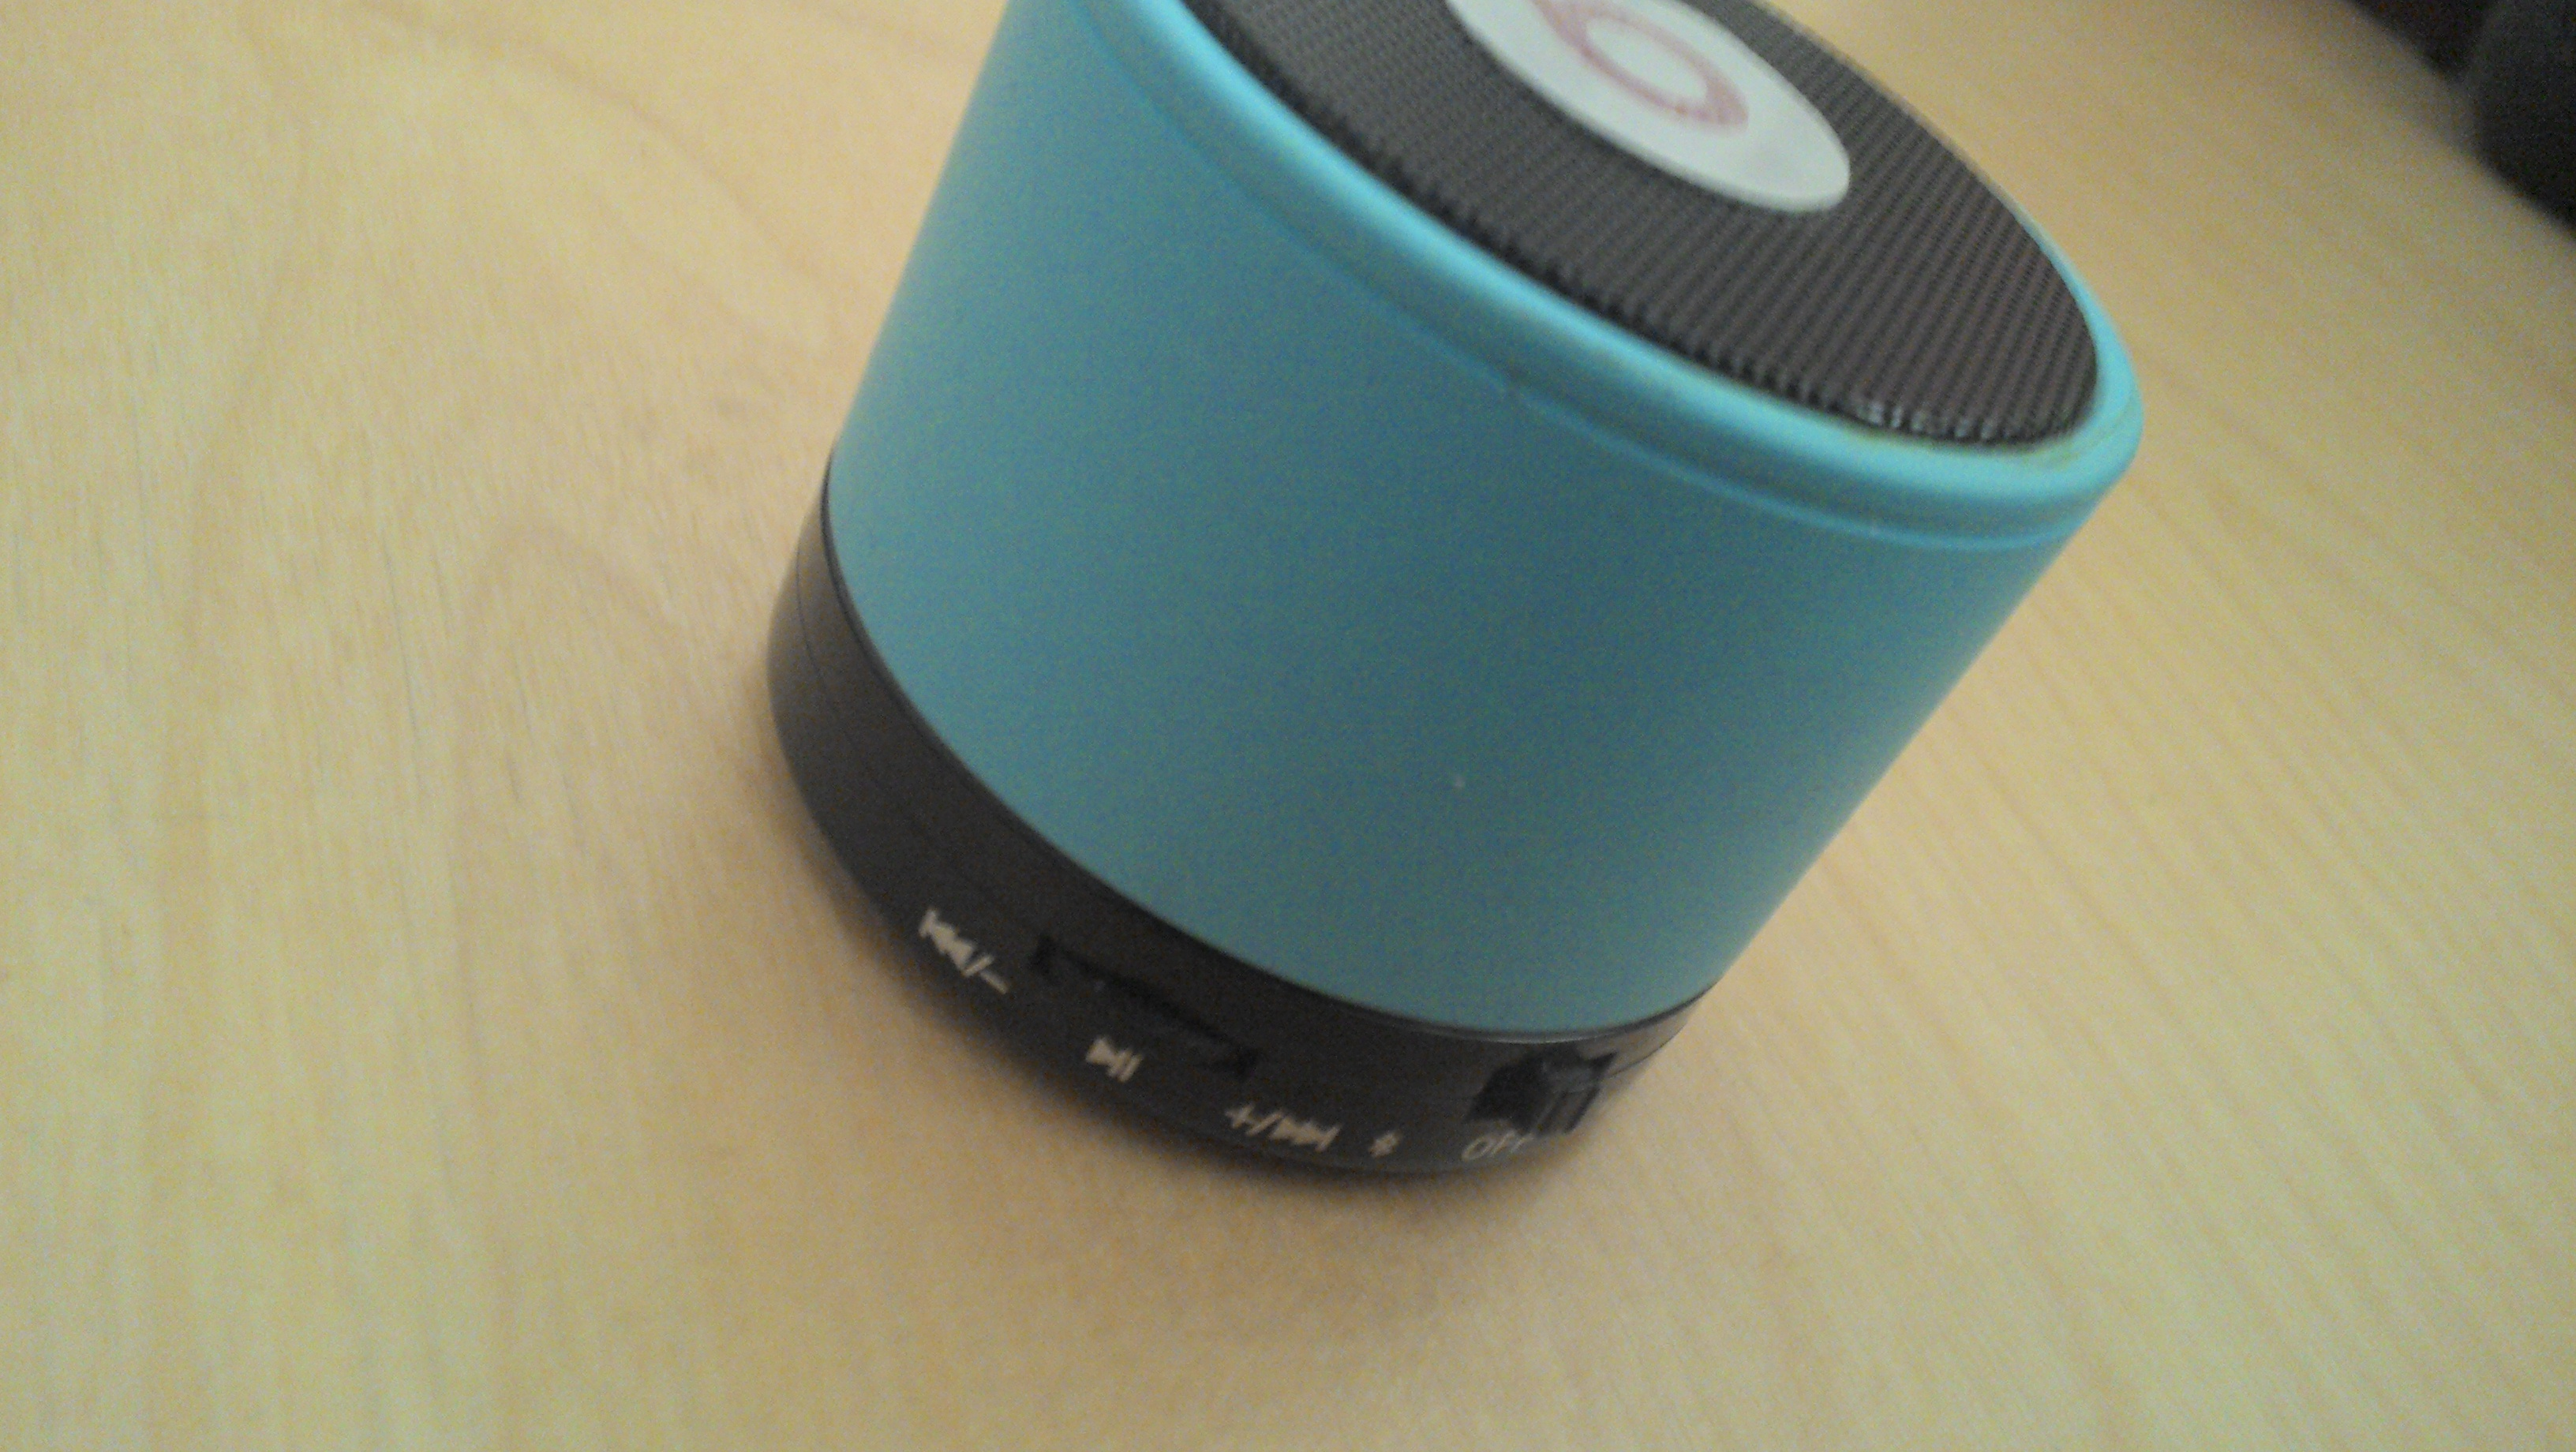
\includegraphics[width=1\textwidth]{pic2.jpg}
\label{fig:wwu_logo}
\end{figure}

\textbf{Beschreibung:} Mobiler Lautsprecher/MP3-Player von Beats. Enthält alle Standard-Feature wie Lautstärke-Regler, Pause/Play-Button, Vorheriger/Nächster Track-Button. Erlaubt die Verbindung per Bluetooth und das Einstecken einer Speicherkarte. 
\\
\\
\\
\textbf{Funktionalität:} Leichte Verbindung mit ausreichender Reichweite. Akku hält für einige Stunden und das Gerät funktioniert, auch während es an einer Stromversorgung hängt. Allerdings ist es nicht sehr sicher: Jeder im Bluetooth-Umkreis kann sich mit dem Gerät verbinden und bisher verbundene Datenträger verdrängen, da es keinen Paring-Button oder ähnliches gibt.
\\
\textbf{Ergonomie:} Da der Lautsprecher nach oben zeigt, ist die Soundqualität in jede Richtung gleich gut. Dadurch wird das Gerät in der Regel in die Mitte einer Gruppe von Leuten platziert und erhält viel Aufmerksamkeit. Die oben beschriebenen Standard-Feature sind in einem einzigen Regler kombiniert (eindrücken für Pause/Play, in eine Richtung halten für Lautstärke-Regelung, schnell in eine Richtung über den Regler streichen, um den Track zu wechseln). Dadurch erreicht man alle Funktionen, ohne die eigenen Finger viel bewegen oder das Gerät gar in der Hand drehen zu müssen. Außerdem ist der Wechsel zwischen Bluetooth und Speicherkarte in einem 3-Punkt-Schalter, wobei der mittlere Punkt des Schalters das Gerät abschaltet. So muss man nur beim Abschalten des Gerätes Genauigkeit benutzen und kann während des Betriebs einfach den Schalter mit voller Kraft durchdrücken.
\\
\textbf{Symbolik:} Keine religiöse Bewandtnis, aber ein Status-Symbol dank der Beats Marke, die prominent auf der Oberseite dargestellt wird. Gruppenzugehörigkeit durch das Gerät hält sich in Grenzen, da man nicht erwartet, dass jeder permanent einen mobilen Lautsprecher bei sich trägt(anders als ein Smartphone). Außerdem ist das Gerät schon viele Jahre alt, wodurch die Symbolik abermals leidet.
\\
\textbf{Ästhetik:} Es gibt nur sehr wenig Text auf dem Gerät und dieser ist auch noch komplett auf die Basis des Gerätes beschränkt ist. Durch die Bündelung der Funktionen auf nur einen Regler und einen Schalter lässt sich die benötigte Fläche an Text noch weiter verkleinern. Außerdem sind die Seitenflächen komplett einfarbig und ohne Text. Durch diese Beiden Tatsachen hat das Gerät ein sehr schlichtes Design, das dennoch freundlich für neue Benutzer ist (KISS-Prinzip). Das Markenzeichen auf der oberen Fläche hat Züge von der goldenen Spirale. Alle erhältlichen Farbvarianten sind sehr hell, wodurch es zu einem Kontrast mit den schwarzen Flächen an der Basis und an der oberen Seite des Gerätes kommt.
\\
\textbf{Erlebnishaftigkeit:} Es gibt eine LED rechts neben den Reglern des Gerätes. Diese LED gibt durch ihre Farbe und Intervall-Dauer an, in welchem Zustand sich das Gerät befindet (Standby/Aktiv-Modus, Verbindungsaufbau und Akkustand). Die wahrscheinlich wichtigste Funktion der LED ist die Nachricht auf geringen Akkustand. Dies wird durch ein permanentes, rotes Blinken dargestellt. Da wir darauf trainiert sind, dass rote Lichter eine negative Konnotation haben (meist im direkten Bezug auf Akkustand), und da eine blinkende Lampe sehr einfach die Aufmerksamkeit auf sich lenkt, ist dies eine sehr sinnvolle Methode, den Benutzer direkt auf ein Problem hinzuweisen.

\end{document}
